% Bioinformatics, Applications Note. Typeset to follow the journal's layout
% (OUP's bioinformatics.cls is not distributed with TeX Live): two columns,
% structured abstract, author-year citations, four pages.
\documentclass[9pt,twocolumn,a4paper]{extarticle}
\usepackage[top=2.2cm,bottom=2.2cm,left=1.8cm,right=1.8cm,columnsep=0.7cm,headheight=12pt,headsep=0.5cm]{geometry}
\usepackage[T1]{fontenc}
\usepackage{mathptmx}
\usepackage[scaled=0.88]{helvet}
\usepackage{microtype}
\usepackage{graphicx}
\usepackage{booktabs}
\usepackage{makecell}
\usepackage{amssymb}
\usepackage{xcolor}
\usepackage{fancyhdr}
\usepackage{titlesec}
\usepackage{caption}
\usepackage{url}
\usepackage[hidelinks]{hyperref}

\definecolor{oup}{HTML}{1F3E7A}
\newcommand{\code}[1]{{\small\texttt{#1}}}
\captionsetup{font={small},labelfont=bf,labelsep=period,justification=raggedright,singlelinecheck=false}
\setlength{\parindent}{0.9em}
\setlength{\parskip}{0pt}
\linespread{1.0}
\titleformat{\section}{\normalfont\sffamily\bfseries\normalsize\color{oup}}{\thesection}{0.6em}{}
\titleformat{\subsection}{\normalfont\sffamily\bfseries\small}{\thesubsection}{0.6em}{}
\titlespacing*{\section}{0pt}{1.1ex}{0.6ex}
\titlespacing*{\subsection}{0pt}{0.9ex}{0.4ex}

\pagestyle{fancy}\fancyhf{}
\renewcommand{\headrulewidth}{0pt}
\fancyhead[L]{\sffamily\footnotesize Swargo {\it et al.}}
\fancyhead[R]{\sffamily\footnotesize adaptiSeq}
\fancyfoot[C]{\sffamily\footnotesize\thepage}
\fancypagestyle{first}{\fancyhf{}\renewcommand{\headrulewidth}{0pt}%
  \fancyhead[L]{\sffamily\footnotesize Bioinformatics, 2026, 1--4\\ Advance Access Publication Date: 2026\\ Applications Note}%
  \fancyfoot[C]{\sffamily\footnotesize\thepage}}

\makeatletter
\begin{document}
\thispagestyle{first}

\twocolumn[
\begin{@twocolumnfalse}
{\sffamily\footnotesize\color{oup}\textbf{Sequence analysis}}\par\vspace{-1pt}
{\sffamily\bfseries\fontsize{17}{20}\selectfont adaptiSeq: complete, verified download of public sequencing accession lists}\par\vspace{6pt}
{\sffamily\bfseries\small Rasman Mubtasim Swargo$^{1}$, Nieb Hasan Neom$^{1}$ and Md Arifuzzaman$^{1,*}$}\par\vspace{3pt}
{\footnotesize $^{1}$Department of Computer Science, Missouri University of Science and Technology, Rolla, MO, USA\\
$^{*}$To whom correspondence should be addressed. E-mail: marifuzzaman@mst.edu\\
Associate Editor: XXXXXXX\par\vspace{1pt}
Received on XXXXX; revised on XXXXX; accepted on XXXXX}\par\vspace{4pt}
\hrule\vspace{5pt}
{\small
\noindent\textsf{\textbf{Abstract}}\\
\textbf{Summary:} Reanalysis of public sequencing data starts from a list of accessions, often hundreds of runs. Existing downloaders fetch such a list one run at a time over one connection, and some report success while runs are missing or were silently replaced by files that cannot be checked against the archive. adaptiSeq is a Python library and command-line tool, a reimplementation of iSeq, that resolves accessions from GSA, SRA, ENA, DDBJ and GEO in parallel under per-archive request limits, downloads files as resumable byte ranges over many connections, checks every file against the archive's MD5 as it lands, and exits non-zero when a run is not delivered. On a 241-run ENA project, the fastest other tool that delivered every run was 6.1 times slower than adaptiSeq with default settings in the median repetition; adaptiSeq never exited 0 with a run missing, against 8 of 40 benchmark rows for iSeq, Kingfisher and fastq-dl. Resolution, transfer and verification are also available as Python functions, and several controllers for the number of concurrent files are built in.\par\vspace{3pt}
\textbf{Availability and implementation:} adaptiSeq is written in Python ($\ge$3.10) and released under the MIT licence at \url{https://github.com/swargo98/adaptiSeq} and \url{https://pypi.org/project/adaptiseq/}. Benchmark scripts, accession lists and result tables are in the repository.\par\vspace{3pt}
\textbf{Contact:} \href{mailto:marifuzzaman@mst.edu}{marifuzzaman@mst.edu}\par\vspace{3pt}
\textbf{Supplementary information:} Supplementary data are available at \textit{Bioinformatics} online.}
\vspace{3pt}\hrule\vspace{8pt}
\end{@twocolumnfalse}
]

\section{Introduction}
The Sequence Read Archive (SRA; Katz {\it et al.}, 2022), the European Nucleotide Archive (ENA; Yuan {\it et al.}, 2026), the DDBJ Sequence Read Archive (Ara {\it et al.}, 2026) and the Genome Sequence Archive (GSA; Chen {\it et al.}, 2021) hold tens of millions of sequencing runs, and reanalysis of deposited runs is routine. The unit of work is rarely one file: a pipeline is given a project or a list of run accessions and must obtain every run, intact, before analysis can start.

Several tools download by accession. iSeq (Chao {\it et al.}, 2024) covers five databases with one command-line interface and verifies checksums. Kingfisher (Woodcroft {\it et al.}, 2024) tries several sources for each run, fastq-dl (Petit {\it et al.}, 2026) retrieves FASTQ files from ENA or SRA, nf-core/fetchngs (Patel {\it et al.}, 2026; Ewels {\it et al.}, 2020) wraps retrieval in a Nextflow workflow, and pysradb (Choudhary, 2019) exposes metadata and downloads to Python. Apart from fetchngs and pysradb with a thread count, these tools handle the runs of a list sequentially. That matters because ENA serves each TCP connection at only a few MB/s, so one connection leaves most of the path idle. It also matters because archive services fail in ways that tools can mistake for an answer. In a 17-day probe of the ENA portal API from a compute node, 3.1\% of 3,420 queries failed outright, and a tool that reads a failed query as ``run not in ENA'' falls back to another source whose files cannot be checked against ENA's checksum.

We present adaptiSeq, a Python reimplementation and extension of iSeq built for accession lists. It keeps iSeq's database coverage, options and integrity checks, and changes how the bytes arrive: concurrent resolution, a segmented and resumable transfer engine ported from FastBioDL (Swargo {\it et al.}, 2025), in-pool checksum verification, and an exit status that reflects what was delivered.

\section{Implementation}
\textbf{Resolution.} Run metadata and file locations are obtained in iSeq's order: the ENA Portal API, NCBI for runs ENA does not mirror, and the GSA interfaces for CRA/CRR accessions. Lookups for a list run in a thread pool (\code{--meta-jobs}), each endpoint behind its own request limiter (8 requests/s for ENA, 5 for GSA, 3 for NCBI, 10 with an API key). A failed ENA query is retried with backoff and is not read as ``not in ENA'' until about three minutes of continuous failure; any fallback to SRA is announced, recorded as unverified, and can be refused (\code{--no-sra-fallback}).

\textbf{Transfer.} The resolved files form one queue served by up to \code{-j} workers (default 20). Each file is split into byte ranges (one per 512~MiB, at most eight), fetched over HTTPS where the host honours ranges and otherwise over FTP, and written at its offset into a \code{.part} file with progress in a sidecar, so an interrupted transfer resumes per range. Idle connections take over the remainder of the largest outstanding range, so connections stay busy until the last byte. A per-host guard reads a refused connection while others are open as a ceiling to wait at, and halves its limit only on HTTP 429/503.

\textbf{Integrity.} Each finished file is hashed inside the worker pool and compared with the MD5 the archive publishes; a mismatching file is deleted and re-queued, so a corrupt copy is fetched again in parallel with the rest of the list. A run that cannot be verified after three rounds is written to \code{fail.log} and the exit status is non-zero. Runs with three FASTQ files are downloaded and verified in full.

\textbf{Interfaces.} The command line follows iSeq's (\code{adaptiseq -i accessions.txt -g}). The same operations are importable, return values and raise typed exceptions, and work inside a running event loop:
\begin{center}\small\ttfamily\begin{minipage}{0.93\columnwidth}\raggedright
from adaptiseq import fetch, get\_metadata\\
rows = get\_metadata("PRJNA916347")\\
res = fetch("accessions.txt", outdir="d", gzip=True)\\
if res.failed: print(res.fail\_ids)
\end{minipage}\end{center}
adaptiSeq also includes five controllers for the number of files in flight (\code{--controller}); the default searches downward from \code{-j} and commits to the count with the highest measured throughput, and the others (e.g.\ one that uses the fewest connections) are available to users with other goals. Table~1 compares adaptiSeq with the other tools.

\begin{figure*}[!t]
\centering
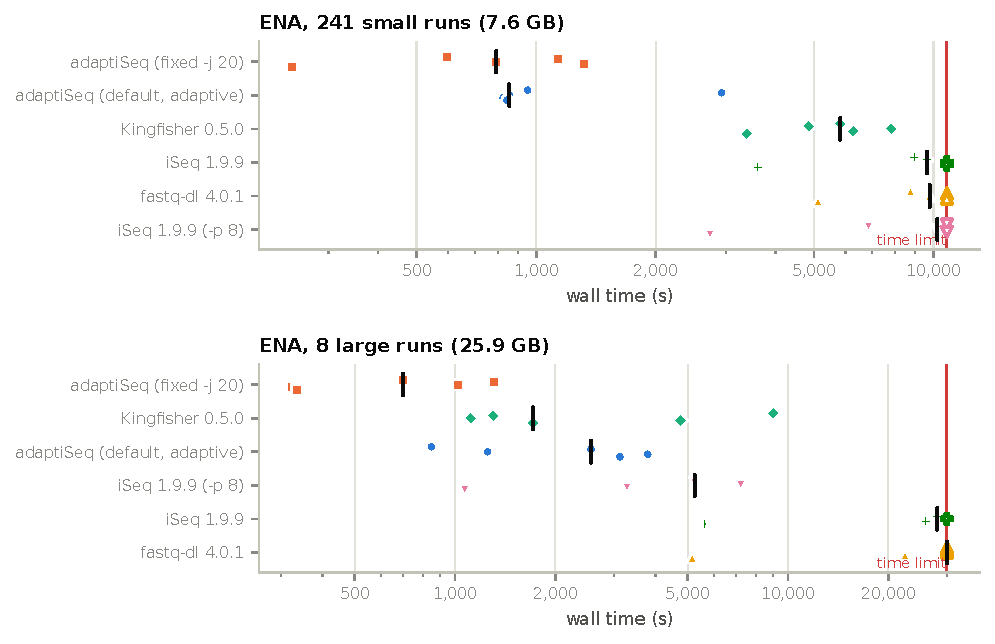
\includegraphics[width=0.485\textwidth]{figs/chain_wall.pdf}\hfill
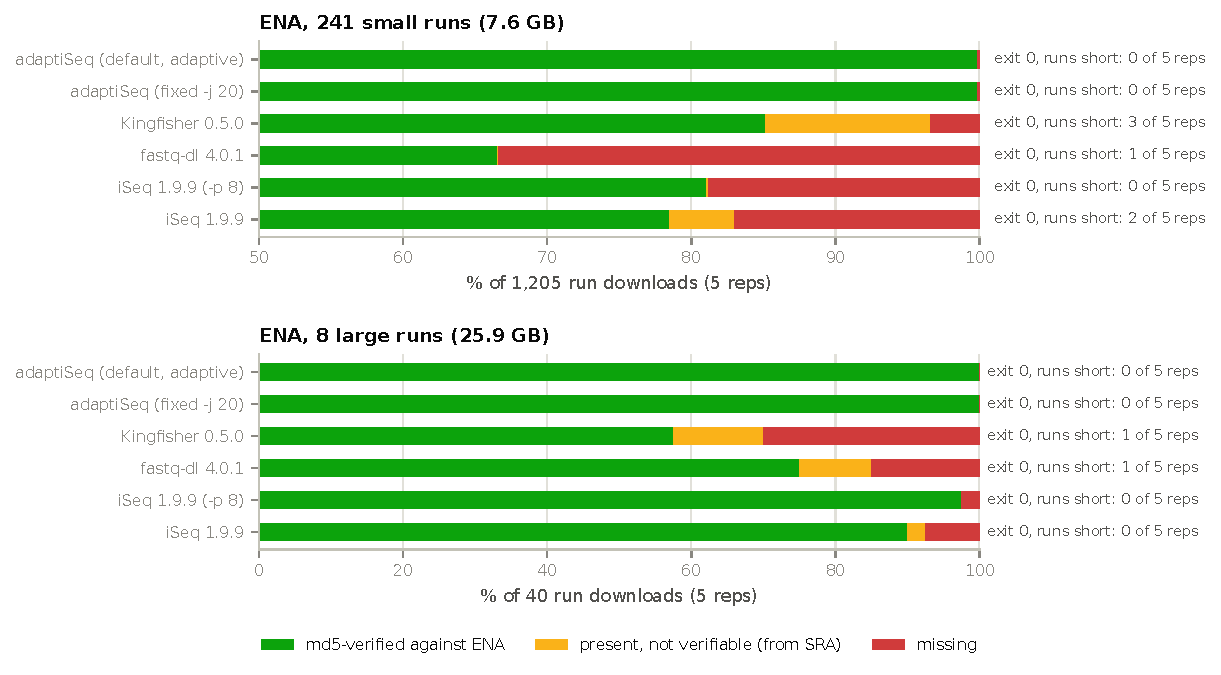
\includegraphics[width=0.505\textwidth]{figs/chain_complete.pdf}
\caption{Five repetitions of two ENA lists on SDSC Expanse. \textbf{(a)} Wall time of every arm, small runs (top, 241 runs) and large runs (bottom, 8 runs); filled markers finished, hollow markers reached the time limit (lower bounds), bars are medians, the horizontal axis is logarithmic. \textbf{(b)} Run downloads over five repetitions split into MD5-verified against ENA, present but not verifiable (fetched from SRA and converted), and missing; the right-hand notes count repetitions in which the tool exited 0 although runs were short.}\label{fig:main}
\end{figure*}

\begin{table}[!t]
\caption{Feature comparison, from each tool's help output, source and documentation at the versions shown.}\label{tab:feat}
\setlength{\tabcolsep}{2.3pt}\renewcommand{\arraystretch}{1.08}
\centering{\scriptsize
\begin{tabular}{@{}lcccccc@{}}
\toprule
 & \makecell{adapti-\\Seq\\0.1.12} & \makecell{iSeq\\1.9.9} & \makecell{King-\\fisher\\0.5.0} & \makecell{fastq-\\dl\\4.0.1} & \makecell{fetch-\\ngs\\1.13.0} & \makecell{pysra-\\db\\2.5.1}\\
\midrule
Accession list in one call & \checkmark & \checkmark & \checkmark & -- & \checkmark & project\\
Several runs at once & \checkmark & -- & -- & -- & \checkmark & \checkmark\\
Rate-limited parallel resolution & \checkmark & -- & -- & -- & no cap & --\\
MD5 check & \checkmark & \checkmark & optional & \checkmark & \checkmark & --\\
Resume partial file & \checkmark & \checkmark & -- & -- & task & \checkmark\\
Merge runs & \checkmark & \checkmark & -- & \checkmark & -- & --\\
Python API & \checkmark & -- & \checkmark & -- & -- & \checkmark\\
GSA / GEO & \checkmark/\checkmark & \checkmark/\checkmark & exp./-- & --/-- & --/\checkmark & --/\checkmark\\
\bottomrule
\end{tabular}}
\end{table}

\section{Benchmark}
We compared adaptiSeq 0.1.12 with iSeq 1.9.9 (default, and \code{-p 8}), Kingfisher 0.5.0 and fastq-dl 4.0.1 on two public ENA lists chosen to stress different costs: BioProject PRJNA916347 (241 runs, 321 files, 7.6~GB, 40 runs with three FASTQ files; per-run overhead dominates) and eight runs of PRJNA762469 (16 files, 25.9~GB; bandwidth dominates). Every tool was asked for gzip-compressed FASTQ with checksum verification on. adaptiSeq ran with defaults (\code{adaptiseq -i LIST -g}) and with a fixed pool (\code{--no-adaptive -j 20}). Each arm ran five times on an exclusive node of SDSC Expanse (Strande {\it et al.}, 2021), one arm at a time, in an order drawn afresh for each repetition, with a time limit of 3~h (small runs) or 8.3~h (large runs). Afterwards an independent verifier hashed the output and matched it to a manifest taken from ENA; a run counts as complete only if every file matches, whatever the tool's exit status. Throughput is verified bytes over elapsed time, including resolution and verification. We report medians over repetitions and, for speed, the median of the paired ratio within a repetition.

\textbf{Speed.} On the 241-run list, adaptiSeq's median wall time was 855~s with defaults (8.9~MB/s) and 794~s with the fixed pool (9.5~MB/s) (Fig.~1a). The other tools' medians never exceeded 1.3~MB/s. The fastest other tool that delivered every run was, per repetition, a median of 6.1 times slower than the default and 9.8 times slower than the fixed pool, and the other tools reached the time limit in 6 of 20 rows. On the eight large runs the medians were 2,561~s (10.1~MB/s) for the default and 699~s (37.0~MB/s) for the fixed pool, against 1,715~s (5.4~MB/s) for Kingfisher, the fastest other tool by median; the paired ratio of the default to the fastest complete tool was 5.8, but not in every repetition: in two of five, iSeq \code{-p 8} finished first. The gain comes from connections: adaptiSeq held a median of 15.6 (small runs) and 21.7 (large runs) open connections to ENA, against one for iSeq and fastq-dl and medians of 1.7 and 4.0 for Kingfisher. Fixing the number of files in flight from 1 to 64 shows near-proportional gains up to eight and 15--23 times over one file at a time at the best setting (Supplementary Fig.~S1).


\textbf{Completeness.} adaptiSeq delivered all runs with every file verified in 16 of its 20 rows (Fig.~1b). In the other four, one run of the 241 was missing; ENA's copy of one file failed MD5 three times or could not be opened, adaptiSeq exited 1 and named the run in \code{fail.log}. Over the five repetitions it verified 1,203 of 1,205 small-run downloads and 40 of 40 large-run downloads, never delivered a file it could not check, and never exited 0 with a run missing (0 of 20 rows). iSeq, Kingfisher and fastq-dl verified 67--85\% of small-run downloads and 58--98\% of large-run downloads, exited 0 with runs short in 8 of their 40 rows, and delivered 204 run downloads as files that cannot be checked against ENA's MD5, almost all because ENA's API answered without FASTQ links and the tool fetched the run from SRA instead. ENA also served bad copies: 178 MD5 mismatches appeared in the logs of 44 of 96 benchmark rows, in every tool and on different files in different arms of the same hour, so detecting and re-fetching them in the pool, rather than at the end of a run, is part of the speed as well as the correctness.

\textbf{Reliability.} In separate tests of an earlier build (0.1.3, single-stream transfers, one machine, six trials per tool), adaptiSeq and iSeq both resumed a transfer killed at 25, 50 or 75\% without re-downloading completed bytes; in adaptiSeq a dropped connection never produced a truncated output file and a corrupted byte was detected and repaired (Supplementary Table~S1).

\section{Discussion}
adaptiSeq is aimed at lists, where concurrency across runs and within files, and an exit status that can be trusted, matter more than the speed of one transfer; for a single large file, a multi-connection downloader such as aria2c is likely as fast. Throughput from the archives changed more than tenfold between days (the per-connection rate from our node ranged from 0.5 to 7~MB/s), so absolute numbers describe one site over one week and only paired ratios within a repetition are comparable. A fixed pool of 20 was faster than the adaptive default on most ENA cases (median ratio 1.6 and 2.0 on small and large runs), and the default was held back in some repetitions by a single failed transport probe that sent a whole list to FTP. adaptiSeq is distributed through PyPI and not yet Bioconda, and relies on external programs (\code{wget}; sra-tools and \code{pigz} when conversion is needed).

\section*{Acknowledgements}
adaptiSeq is derived from iSeq (Chao {\it et al.}, 2024) and its transfer engine from FastBioDL (Swargo {\it et al.}, 2025). This work used Expanse at the San Diego Supercomputer Center through allocation CIS250262 from the Advanced Cyberinfrastructure Coordination Ecosystem: Services \& Support (ACCESS) program (Boerner {\it et al.}, 2023), supported by U.S. National Science Foundation grants \#2138259, \#2138286, \#2138307, \#2137603 and \#2138296.

\section*{Funding}
\textit{[Funding statement to be completed by the authors.]}

\section*{Conflict of interest}
None declared.

\section*{Data availability}
Accession lists, checksum manifests, benchmark scripts, raw result tables and the analysis scripts are in the project repository. All sequencing data are public in ENA and SRA.

\vspace{4pt}
{\sffamily\bfseries\small\color{oup}References}\vspace{2pt}
\renewcommand{\refname}{}
\renewcommand\@biblabel[1]{}
\begin{thebibliography}{99}\small
\bibitem[Ara {\it et~al.}(2026)]{ddbj} Ara,T. {\it et~al.} (2026) DDBJ update in 2025: system integration for global data-sharing including pathogen surveillance. {\it Nucleic Acids Res.}, {\bf 54}, D106--D110.
\bibitem[Boerner {\it et~al.}(2023)]{access} Boerner,T.J. {\it et~al.} (2023) ACCESS: advancing innovation. In {\it Practice and Experience in Advanced Research Computing (PEARC '23)}, pp. 173--176.
\bibitem[Chao {\it et~al.}(2024)]{iseq} Chao,H. {\it et~al.} (2024) iSeq: an integrated tool to fetch public sequencing data. {\it Bioinformatics}, {\bf 40}, btae641.
\bibitem[Chen {\it et~al.}(2021)]{gsa} Chen,T. {\it et~al.} (2021) The Genome Sequence Archive Family: toward explosive data growth and diverse data types. {\it Genomics Proteomics Bioinformatics}, {\bf 19}, 578--583.
\bibitem[Choudhary(2019)]{pysradb} Choudhary,S. (2019) pysradb: a Python package to query next-generation sequencing metadata and data from NCBI Sequence Read Archive. {\it F1000Research}, {\bf 8}, 532.
\bibitem[Ewels {\it et~al.}(2020)]{nfcore} Ewels,P.A. {\it et~al.} (2020) The nf-core framework for community-curated bioinformatics pipelines. {\it Nat. Biotechnol.}, {\bf 38}, 276--278.
\bibitem[Katz {\it et~al.}(2022)]{sra} Katz,K. {\it et~al.} (2022) The Sequence Read Archive: a decade more of explosive growth. {\it Nucleic Acids Res.}, {\bf 50}, D387--D390.
\bibitem[Patel {\it et~al.}(2026)]{fetchngs} Patel,H. {\it et~al.} (2026) nf-core/fetchngs v1.13.0. Zenodo, doi:10.5281/zenodo.22764959.
\bibitem[Petit {\it et~al.}(2026)]{fastqdl} Petit,R.A. III {\it et~al.} (2026) fastq-dl: efficiently download FASTQ files from SRA or ENA repositories, v4.0.1. Zenodo, doi:10.5281/zenodo.8051230.
\bibitem[Strande {\it et~al.}(2021)]{expanse} Strande,S. {\it et~al.} (2021) Expanse: computing without boundaries. In {\it Practice and Experience in Advanced Research Computing (PEARC '21)}, pp. 1--4.
\bibitem[Swargo {\it et~al.}(2025)]{fastbiodl} Swargo,R.M., Arslan,E. and Arifuzzaman,M. (2025) Adaptive parallel downloader for large genomic datasets. arXiv:2508.05511.
\bibitem[Woodcroft {\it et~al.}(2024)]{kingfisher} Woodcroft,B.J. {\it et~al.} (2024) Kingfisher: a utility for procurement of public sequencing data. Zenodo, doi:10.5281/zenodo.10525085.
\bibitem[Yuan {\it et~al.}(2026)]{ena} Yuan,D. {\it et~al.} (2026) The European Nucleotide Archive in 2025. {\it Nucleic Acids Res.}, {\bf 54}, D120--D127.
\end{thebibliography}


\clearpage
\onecolumn
{\sffamily\bfseries\large\color{oup} Supplementary data}\par\vspace{4pt}
\noindent {\small Supplementary material to ``adaptiSeq: complete, verified download of public sequencing accession lists''. Submitted as a separate file with the journal. Full methodology, every benchmark row and the per-campaign figures are in the repository (\code{plans\_and\_experiments/paper/methodology}).}\par\vspace{8pt}

\begin{figure}[h]\centering
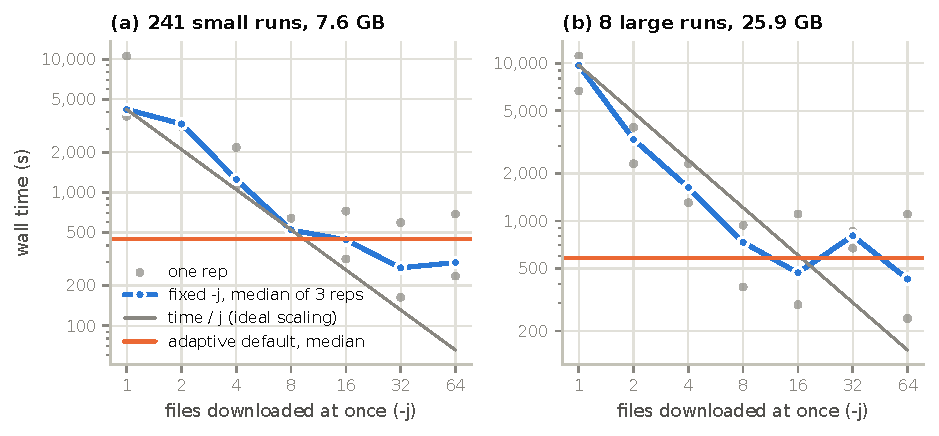
\includegraphics[width=0.7\textwidth]{figs/jsweep.pdf}
\caption*{\textbf{Supplementary Fig. S1.} Wall time against the number of files in flight, fixed \code{-j} from 1 to 64 (build 0.1.7, three repetitions; grey dots are single repetitions, blue is the median, the grey line is perfect scaling from \code{-j}~1, the orange line is the adaptive default). On the 241-run list, one file at a time took 4,197~s and the best median (\code{-j}~32) 271~s (15 times faster); on the eight large runs, 9,708~s and 428~s (\code{-j}~64; 23 times).}
\end{figure}

\begin{table}[h]\centering\small
\caption*{\textbf{Supplementary Table S1.} Resume after a kill (404~MB file, single stream; build 0.1.3, one 8-core machine, two repetitions per kill point).}
\begin{tabular}{@{}llllll@{}}\toprule
Tool & Killed at & Outcome & Bytes re-downloaded & Final MD5 valid & Trials\\\midrule
adaptiSeq & 25, 50, 75\% & resumed from offset & 0\% & 6/6 & 6\\
iSeq & 25, 50, 75\% & resumed from offset & 0\% & 6/6 & 6\\\bottomrule
\end{tabular}\par\vspace{6pt}
\begin{tabular}{@{}lll@{}}\toprule
Check (adaptiSeq) & Condition & Observed\\\midrule
Never truncate & server without range support & single stream; complete file, MD5 match (2/2)\\
Short read & connection dropped mid-body & truncated \code{.part} never renamed (2/2)\\
Corruption & one byte flipped after download (live ENA) & caught by MD5; re-download valid (1/1)\\
Circuit breaker & synthetic HTTP 429 & host limit halved per trip, backoff 1, 2, 4, 8~s; MD5 valid (2/2)\\\bottomrule
\end{tabular}
\end{table}

\begin{figure}[h]\centering
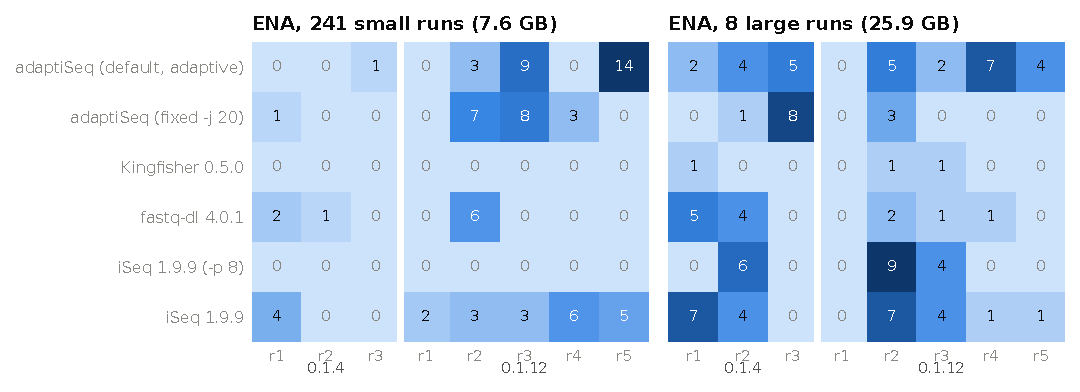
\includegraphics[width=0.8\textwidth]{figs/md5.pdf}
\caption*{\textbf{Supplementary Fig. S2.} MD5 mismatches logged per arm and repetition in the first full run (build 0.1.4, left of each panel) and the final comparison (build 0.1.12, right). Mismatches move between tools and days: they are bad copies or bad transfers at the archive. Counts come from log lines whose wording differs between tools.}
\end{figure}
\end{document}
